\documentclass[a4paper,oneside]{article}
\usepackage[T1]{fontenc}
\usepackage[utf8]{inputenc}
\usepackage[english]{babel}

\usepackage[margin=2.54cm]{geometry}
\usepackage{amsmath}
\usepackage{bbm}
\usepackage{siunitx}
\usepackage{listings}
\usepackage{color}
\usepackage{textcomp}
\usepackage{graphicx}
\usepackage{subcaption}
%\usepackage{changepage}
\usepackage[section]{placeins}
\usepackage{hyperref}

\definecolor{matlabgreen}{RGB}{28,172,0}
\definecolor{matlablilas}{RGB}{170,55,241}

\newcommand{\includecode}[1]{\lstinputlisting[caption={\ttfamily #1.m},label={lst:#1}]{matlab/#1.m}}
\newcommand{\inlinecode}[1]{\lstinline[basicstyle=\ttfamily,keywordstyle={},stringstyle={},commentstyle={\itshape}]{#1}}

\renewcommand{\vec}[1]{\underline{#1}}
\renewcommand{\Re}[1]{\operatorname{Re}\left[#1\right]}
\newcommand{\E}[1]{\operatorname{E}\left[#1\right]}
\newcommand{\norm}[1]{\left\lVert#1\right\rVert}
\newcommand{\abs}[1]{\left|#1\right|}
\newcommand{\F}[1]{\operatorname{\mathcal{F}}\left[#1\right]}
\newcommand{\ceil}[1]{\left\lceil#1\right\rceil}
\newcommand{\floor}[1]{\left\lfloor#1\right\rfloor}
\newcommand{\Prob}[1]{\operatorname{P}\left[#1\right]}
\newcommand{\ProbC}[2]{\operatorname{P}\left[#1\middle|#2\right]}
\newcommand{\ind}[1]{\operatorname{\mathbbm{1}}\left\{#1\right\}}
\newcommand{\distr}[0]{\sim}
\newcommand{\unif}[1]{\mathcal{U}_{#1}}

\newcolumntype{M}{>{$}r<{$}}

\author{Riccardo Zanol}
\title{Homework 2}

\begin{document}
\lstset{
  language=Matlab,
  basicstyle={\ttfamily \footnotesize},
  breaklines=true,
  morekeywords={true,false,warning,xlim,ylim},
  keywordstyle=\color{blue},
  stringstyle=\color{matlablilas},
  commentstyle={\color{matlabgreen} \itshape},
  numberstyle={\ttfamily \tiny},
  frame=leftline,
  showstringspaces=false,
  numbers=left,
  upquote=true,
}
\maketitle
\section*{1}
The function \inlinecode{lcg} implements a Linear Congruential
Generator, which is a RNG than produces a specified number of samples
from the sequence $x_k$, according to the equation
\[ x_{k} = ax_{k-1} +b \mod m  \]
and starting with a given $x_0$.  To replicate Figure~6.5 a LCG with
parameters $a=16807$,~$b=0$~and~$m=2^{31}-1$ is initialized with the
seed value $x_0 = 1$, the first 1000 numbers that it generates are
then sorted and plotted in Fig.~\ref{plot:qqplot}, where they look to
be uniformly distributed in $[0,1]$.  From their autocorrelation
(Fig.~\ref{plot:autocorr}) and their lag plots
(Fig.~\ref{plot:lagplot}) the generated numbers appear to be
uncorrelated.
\begin{figure}[htbp]
  \centering
  \begin{subfigure}{0.5\textwidth}
    \centering
    \includegraphics[width=0.95\textwidth]{matlab/uniform_qq}
    \caption{QQ plot}
    \label{plot:qqplot}
  \end{subfigure}%
  \begin{subfigure}{0.5\textwidth}
        \centering
    \includegraphics[width=0.95\textwidth]{matlab/rand1_autocorr}
    \caption{Autocorrelation}
    \label{plot:autocorr}
  \end{subfigure}
  \begin{subfigure}{0.75\textwidth}
        \centering
    \includegraphics[width=\textwidth]{matlab/rand1_lagplot}
    \caption{Lag plot}
    \label{plot:lagplot}
  \end{subfigure}
  \caption{LCG}
\end{figure}

Using the same LCG to generate two sequences the results are very
different depending on the choice of the seed values: if the two
parallel sequences start with 1 and 2, their output is very correlated
as can be seen in Fig.~\ref{plot:lcg_close_seeds}. If, instead, the
second stream starts from the last value of the first one the two
sequences look independent in Fig.\ref{plot:lcg_far_seeds}.
\begin{figure}[htbp]
  \centering
  \begin{subfigure}{0.5\textwidth}
    \centering
    \includegraphics[width=0.95\textwidth]{matlab/lcg_close_seeds}
    \caption{Parallel streams with close seeds}
    \label{plot:lcg_close_seeds}
  \end{subfigure}%
  \begin{subfigure}{0.5\textwidth}
    \centering
    \includegraphics[width=0.95\textwidth]{matlab/lcg_far_seeds}
    \caption{Parallel streams with no overlap}
    \label{plot:lcg_far_seeds}
  \end{subfigure}
  \caption{Parallel streams}
\end{figure}

To generate a random variable $Y_1$ with p.d.f.
\[ f_{Y_1}(y) = K\frac{\sin^2(y)}{y^2} \qquad -10 \leq y \leq 10 \]
it is possible to use the algorithm based on theorem 6.3 (rejection
sampling for distribution with density), where the upper bound of
$f_{Y_1}^n$ is $M=1$ and the interval where the r.v. $X$ is drawn from
is $[-10,10]$. The histogram of 2000 generated samples of $Y_1$ is
shown in Fig.~\ref{plot:rejection_histo}.
\begin{figure}[htbp]
  \centering
  \begin{subfigure}{0.5\textwidth}
    \centering
    \includegraphics[width=0.95\textwidth]{matlab/rejection_histo}
    \caption{Histogram of $Y_1$}
    \label{plot:rejection_histo}
  \end{subfigure}%
  \begin{subfigure}{0.5\textwidth}
    \centering
    \includegraphics[width=0.95\textwidth]{matlab/rejection_scatter}
    \caption{Generated values of $Y_2$}
    \label{plot:rejection_scatter}
  \end{subfigure}
  \caption{Rejection sampling}
\end{figure}

The other random variable $Y_2$ with p.d.f.
\[ f_{Y_2}(y_1, y_2) = K\abs{y_1 - y_2} \qquad (y_1, y_2) \in [0, 1]^2 \]
can be generated in the same way: the upper bound on $f_{Y_2}^n$ is
$M=1$ also in this case and the random variable $X = (X_1, X_2)$ is
drawn by generating two r.v.s $X_1, X_2 \distr \unif{[0,1]}$. In
Fig.~\ref{plot:rejection_scatter} are shown 2000 samples produced with
this method.
\section*{2}
In Figures \ref{plot:binomial_1}, \ref{plot:binomial_2} and
\ref{plot:binomial_3} there are the times it takes to generate
$N=5\cdot10^4$ Binomial random variables with parameters $n$ and $p$
using three different methods:
\begin{enumerate}
\item By using the algorithm based on the CDF inversion that
  iteratively computes
  \begin{align*}
    \mathrm{pr}(i) &= \Prob{X = i} = \frac{p}{1-p}\frac{n-i}{i+1}\Prob{X = i-1} \\
    F(i) &= F(i-1) + \mathrm{pr}(i) ,
  \end{align*}
  stops as soon as $F(i) > U$, where $U$ is a uniform r.v. in $[0,
    1]$, and takes $x = i$ as the realization of the Binomial r.v.
  \item By generating $n$ Bernoullian r.v.s and counting the number of
    successes, where each Bernoullian $b_i$ is generated from a uniform
    r.v. $U_i$ as $b_i = \ind{U_i \leq p}$.
  \item By generating a string of zeros of length $K_i$, geometrically
    distributed with parameter $p$, counting a one at $K_i+1$ and
    iterating until $\sum_i \left( K_i + 1 \right) > n$. The geometric
    r.v.s are generated, using the CDF inversion method, as
    \[ K_i = \floor{\frac{\ln U_i}{\ln (1 - p)}} . \]
\end{enumerate}
\begin{figure}[htbp]
  \centering
  \begin{subfigure}{0.5\textwidth}
    \centering
    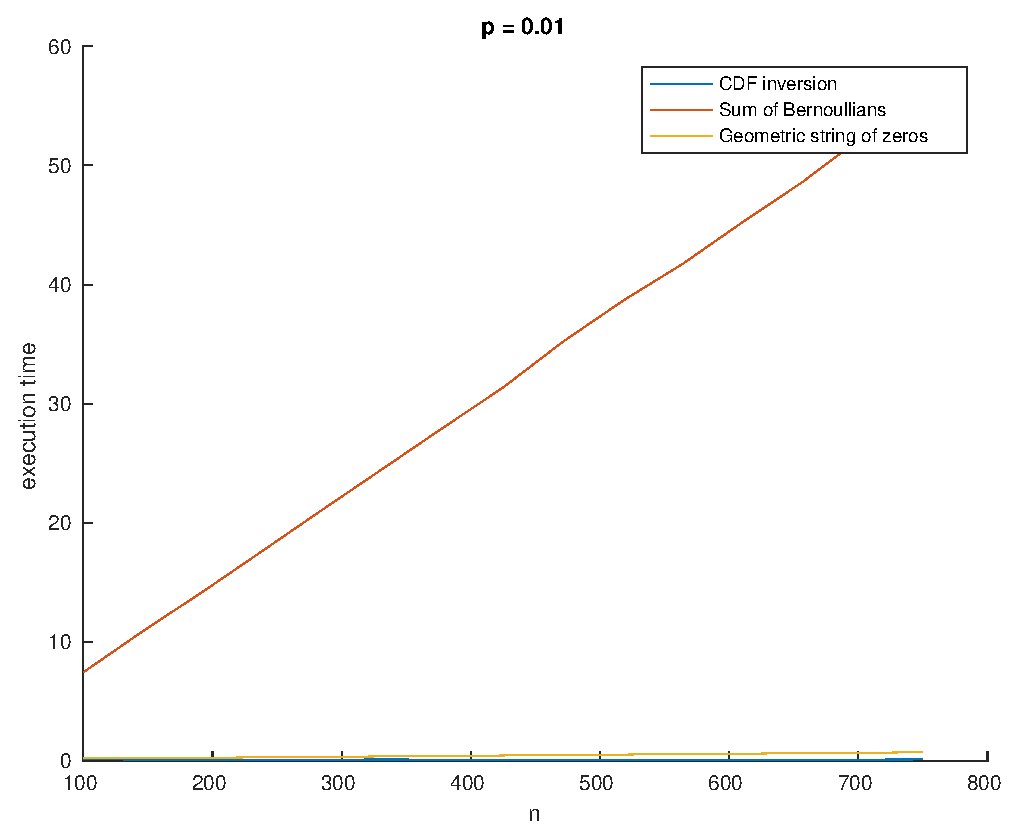
\includegraphics[width=0.95\textwidth]{binomial_gen_1}
    \caption{Succes probability $p=0.01$}
    \label{plot:binomial_1}
  \end{subfigure}%
  \begin{subfigure}{0.5\textwidth}
    \centering
    \includegraphics[width=0.95\textwidth]{binomial_gen_2}
    \caption{Success probability $p=0.5$}
    \label{plot:binomial_2}
  \end{subfigure}
  \begin{subfigure}{0.5\textwidth}
    \centering
    \includegraphics[width=0.95\textwidth]{binomial_gen_3}
    \caption{Success probability $p=0.9$}
    \label{plot:binomial_3}
  \end{subfigure}
  \caption{Performance of the three Binomial generation algorithms}
\end{figure}

In Figures \ref{plot:binomial_1}, \ref{plot:binomial_2} and
\ref{plot:binomial_3} there are the measured execution times for three
diffenrent values of the success probability $p \in \{ 0.01, 0.5, 0.9
\}$ and for $n$ that varies in $[100, 750]$. All the three algorithms
have an execution time that increases linearly with $n$ and the CDF
inversion is always the best algorithm. The first and the second
method do not depend on the value of $p$, but when the samples are
generated with geometric strings of zeros the performnce is very close
to that of the CDF inversion if $p$ is small and moves toward that of
the sum of Bernoullians when $p$ increases. When $p=0.9$ the CDF
inversion algorithm does not terminate because the probability
$\mathrm{pr}(0) = (1-p)^n$ becomes so small, when $n \geq n_{max} =
324$, that Matlab represents it with 0.
\section*{3}
Like in the previous section three methods are used to generate
$N=5\cdot10^4$ samples of a Poisson random variable with parameter
$\lambda$:
\begin{enumerate}
  \item By using the algorithm based on the CDF inversion that
  iteratively computes the distribution function
  \begin{align*}
    F(i) &= F(i-1) + \mathrm{pr}(i) \\
    \mathrm{pr}(i) &= \Prob{X = i} = \frac{\lambda}{i+1}\Prob{X = i-1} , 
  \end{align*}
  where the starting values are $F(0) = \mathrm{pr}(0) =
  e^{-\lambda}$, stops as soon as $F(i) > U$, where $U \distr
  \unif{[0,1]}$, and takes $x = i$ as the realization of the Poisson
  r.v.
  \item By generating the exponentially distributed interarrival times
    of a Poisson process with the same arrival rate $\lambda$ in the
    time interval $[0,1]$ and counting the number of arrivals. The
    exponential r.v.s are generated using the CDF inversion method:
    \[ E_i = -\frac{\ln U_i}{\lambda} \qquad U_i \distr \unif{[0,1]} \]
    and the arrivals are counted until $\sum_i E_i > 1$.
    \item The previous algorithm can be improved: since the value of
      the genrerated Poisson r.v. is
      \[ X = \max\left\{n: \sum_{i=1}^n -\frac{\ln U_i}{\lambda} \leq 1 \right\} \]
      and the inequality is equivalent to
      \[ U_1 U_2 \dots U_n \geq e^{-\lambda} \]
      $X$ can be generated by multiplying uniform r.v.s until their
      product goes below $e^{-\lambda}$.
\end{enumerate}
\begin{figure}[htbp]
  \centering
  \includegraphics[width=0.8\textwidth]{poisson_gen}
  \caption{Performance of the three Poisson r.v. generation algorithms}
  \label{plot:poisson}
\end{figure}

Fig.~\ref{plot:poisson} shows the execution time needed to draw $N$
Poisson random variables with respect to the parameter $\lambda \in
[0.01, 1000]$. Like in the previous section all the three execution
times increase linearly with $\lambda$ and the CDF inversion algorothm
is always the quickest one. The CDF inversion method fails when
$\lambda > \lambda_{max} \approx 745$ because Matlab approximates $\mathrm{pr}(0) =
e^{-\lambda}$ with zero, so the algorithm does not terminate. The
third method improves the execution time but has the same problem of
the CDF inversion when $\lambda$ becomes too large.
\section*{4}
To determine whether the two LCGs with parameters $a_1 = 18, b=0,
m=101$ and $a_2 = 2, b=0, m=101$ are full period it is necessary to
generate a sequence of $m-1$ random numbers starting from every
possible seed value $x_0 \in [1, m-1]$ and check that each one of the
sequences has no repeated values. Running this test these two LCGs are
determined to be full period.

If the sequence $u_1(i)$ generated by the first LCG with seed value 1
is plotted together with its shifted version $u_1(i+1)$ it can be seen
in Fig.~\ref{plot:lcg1_scatter} that the pairs $(u_1(i), u_1(i+1))$
are aligned along many parallel lines but they look to be spread
uniformly over the square $[0,1]^2$ so this LCG could be used to draw
two independent sequences. The other LCG is much worse since the
generated couples $(u_2(i), u_2(i+1))$ are all placed on two lines
(see Fig.~\ref{plot:lcg2_scatter}) and do not look random at all.
\begin{figure}[htbp]
  \centering
  \begin{subfigure}{0.5\textwidth}
    \centering
    \includegraphics[width=0.95\textwidth]{matlab/lcg1_scatter}
    \caption{Parameters $a_1 = 18, b=0, m=101$}
    \label{plot:lcg1_scatter}
  \end{subfigure}%
  \begin{subfigure}{0.5\textwidth}
    \centering
    \includegraphics[width=0.95\textwidth]{matlab/lcg2_scatter}
    \caption{Parameters $a_2 = 2, b=0, m=101$}
    \label{plot:lcg2_scatter}
  \end{subfigure}
  \caption{Successive couples generated by two LCGs}
\end{figure}

\end{document}
